\documentclass[tikz]{standalone}

\usetikzlibrary{decorations.pathreplacing} % Pour le bottleneck

\begin{document}
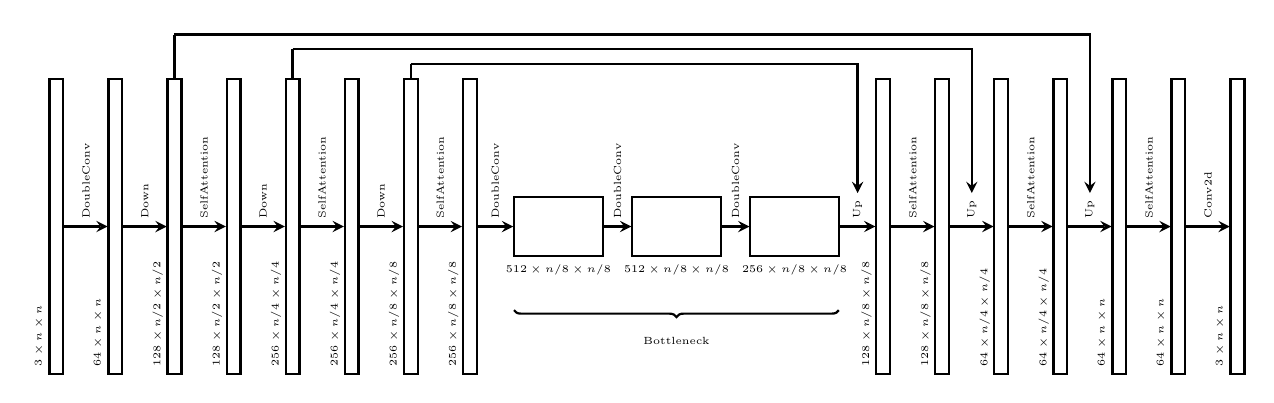
\begin{tikzpicture}[>=stealth, thick, scale=0.75, every node/.style={scale=0.75}]
    \node[draw, minimum height=5cm] (0) at (0, 0) {};
    \node[rotate=90, anchor=north west] (0label) at (-0.5, -2.5) {\tiny $3 \times n \times n$};

    \node[draw, minimum height=5cm] (1) at (1, 0) {};
    \node[rotate=90, anchor=north west] (1label) at (.5, -2.5) {\tiny $64 \times n \times n$};

    \node[draw, minimum height=5cm] (2) at (2, 0) {};
    \node[rotate=90, anchor=north west] (2label) at (1.5, -2.5) {\tiny $128 \times n/2 \times n/2$};

    \node[draw, minimum height=5cm] (3) at (3, 0) {};
    \node[rotate=90, anchor=north west] (3label) at (2.5, -2.5) {\tiny $128 \times n/2 \times n/2$};

    \node[draw, minimum height=5cm] (4) at (4, 0) {};
    \node[rotate=90, anchor=north west] (4label) at (3.5, -2.5) {\tiny $256 \times n/4 \times n/4$};

    \node[draw, minimum height=5cm] (5) at (5, 0) {};
    \node[rotate=90, anchor=north west] (5label) at (4.5, -2.5) {\tiny $256 \times n/4 \times n/4$};

    \node[draw, minimum height=5cm] (6) at (6, 0) {};
    \node[rotate=90, anchor=north west] (6label) at (5.5, -2.5) {\tiny $256 \times n/8 \times n/8$};

    \node[draw, minimum height=5cm] (7) at (7, 0) {};
    \node[rotate=90, anchor=north west] (7label) at (6.5, -2.5) {\tiny $256 \times n/8 \times n/8$};

    \node[draw, minimum height=1cm, minimum width=1.5cm, label={below:\tiny $512 \times n/8 \times n/8$}] (8) at (8.5, 0) {};
    \node[draw, minimum height=1cm, minimum width=1.5cm, label={below:\tiny $512 \times n/8 \times n/8$}] (9) at (10.5, 0) {};
    \node[draw, minimum height=1cm, minimum width=1.5cm, label={below:\tiny $256 \times n/8 \times n/8$}] (10) at (12.5, 0) {};
    \draw[decoration={brace, mirror, raise=.5cm}, decorate] (7.75, -.75) -- node[below, yshift=-1cm] {\tiny Bottleneck} (13.25, -.75);

    \node[draw, minimum height=5cm] (11) at (14, 0) {};
    \node[rotate=90, anchor=north west] (11label) at (13.5, -2.5) {\tiny $128 \times n/8 \times n/8$};

    \node[draw, minimum height=5cm] (12) at (15, 0) {};
    \node[rotate=90, anchor=north west] (12label) at (14.5, -2.5) {\tiny $128 \times n/8 \times n/8$};

    \node[draw, minimum height=5cm] (13) at (16, 0) {};
    \node[rotate=90, anchor=north west] (13label) at (15.5, -2.5) {\tiny $64 \times n/4 \times n/4$};

    \node[draw, minimum height=5cm] (14) at (17, 0) {};
    \node[rotate=90, anchor=north west] (14label) at (16.5, -2.5) {\tiny $64 \times n/4 \times n/4$};

    \node[draw, minimum height=5cm] (15) at (18, 0) {};
    \node[rotate=90, anchor=north west] (15label) at (17.5, -2.5) {\tiny $64 \times n \times n$};

    \node[draw, minimum height=5cm] (16) at (19, 0) {};
    \node[rotate=90, anchor=north west] (16label) at (18.5, -2.5) {\tiny $64 \times n \times n$};

    \node[draw, minimum height=5cm] (17) at (20, 0) {};
    \node[rotate=90, anchor=north west] (16label) at (19.5, -2.5) {\tiny $3 \times n \times n$};


    % inc
    \draw[->] (0) -- node[right, rotate=90] {\tiny DoubleConv} (1);
    % down1
    \draw[->] (1) -- node[right, rotate=90] {\tiny Down} (2);
    % sa1
    \draw[->] (2) -- node[right, rotate=90] {\tiny SelfAttention} (3);
    % down2
    \draw[->] (3) -- node[right, rotate=90] {\tiny Down} (4);
    % sa2
    \draw[->] (4) -- node[right, rotate=90] {\tiny SelfAttention} (5);
    % down3
    \draw[->] (5) -- node[right, rotate=90] {\tiny Down} (6);
    % sa3
    \draw[->] (6) -- node[right, rotate=90] {\tiny SelfAttention} (7);
    % bot1
    \draw[->] (7) -- node[right, rotate=90] {\tiny DoubleConv} (8);
    % bot2
    \draw[->] (8) -- node[right, rotate=90] {\tiny DoubleConv} (9);
    % bot3
    \draw[->] (9) -- node[right, rotate=90] {\tiny DoubleConv} (10);
    % up1
    \draw[->] (10) -- node[right, rotate=90] (up1) {\tiny Up} (11);
    % sa4
    \draw[->] (11) -- node[right, rotate=90] {\tiny SelfAttention} (12);
    % up2
    \draw[->] (12) -- node[right, rotate=90] (up2) {\tiny Up} (13);
    % sa5
    \draw[->] (13) -- node[right, rotate=90] {\tiny SelfAttention} (14);
    % up3
    \draw[->] (14) -- node[right, rotate=90] (up3) {\tiny Up} (15);
    % sa6
    \draw[->] (15) -- node[right, rotate=90] {\tiny SelfAttention} (16);
    % outc
    \draw[->] (16) -- node[right, rotate=90] {\tiny Conv2d} (17);

    \node at (2, 3.25) (l0) {};
    \draw (2.north) -- (l0.center);
    \draw[->] (l0.center) -| (up3.east);

    \node at (4, 3) (l1) {};
    \draw (4.north) -- (l1.center);
    \draw[->] (l1.center) -| (up2.east);

    \node at (6, 2.75) (l2) {};
    \draw (6.north) -- (l2.center);
    \draw[->] (l2.center) -| (up1.east);
\end{tikzpicture}
\end{document}